\documentclass[12pt, a4paper]{article}

\usepackage[default]{sourcesanspro}
\usepackage[T1]{fontenc}
\usepackage[french]{babel}
\usepackage[autolanguage]{numprint}
\usepackage{hyperref}
\usepackage{graphicx}
\usepackage{array}
\usepackage{multirow}
\usepackage{colortbl}
\usepackage{tikz}
\hypersetup{
    colorlinks=true,
    linkcolor=black,
    urlcolor=red,
    pdftitle={NLP Lab3 Report},
}
\usepackage{geometry}
\geometry{left=0.5in, right=0.5in, top=0.5in, bottom=1in}
\usepackage{setspace}
\onehalfspacing
\usepackage[language=french]{lipsum}
\usepackage{mfirstuc}  % For capitalizing words
\usepackage{titlesec}   % For title formatting
\usepackage{ragged2e}
\usepackage{float}

\begin{document}
\begin{titlepage}

\newgeometry{left=0.5in, right=0.5in, top=0.5in, bottom=0.5in}


\begin{minipage}[t]{\linewidth}
\centering
\capitalisewords{République Algerienne Démocratique et Populaire} \\
\capitalisewords{Ministère de l'enseignement supérieur et de la recherche scientifique} \\
\capitalisewords{École supérieure en informatique 8 Mai 1945 Sidi Bel-Abbés} \\
\end{minipage}
\vspace{12pt}
\hrule


\vspace{4cm}

\begin{center}

\vspace{2.5cm}


\huge{\capitalisewords{NLP Lab 3 Report}}

\vspace{0.5cm}

\normalsize
\uppercase{\textbf{Benyamina Yacine Lazreg}}
\normalsize
\uppercase{\textbf{IASD - G01}}

\texttt{
\href{mailto:yl.benyamina@esi-sba.dz}{yl.benyamina@esi-sba.dz}
}

\today

\vspace{2.5cm}


\vfill

\large
2023 - 2024 \\
%\vspace{8pt}
%\hrule


\end{center}
\end{titlepage}


\thispagestyle{empty}
\clearpage

\section*{Named Entity Recognition with GRU}

This report is about implementing a Named Entity Recognition (NER) task using a Gated Recurrent Unit (GRU) model and the CoNLL-2003 dataset. The code performs the following steps:

\begin{enumerate}
    \item \textbf{Data Loading and Preprocessing}: The CoNLL-2003 dataset was loaded, preprocesses the text data by lowercasing and lemmatizing the tokens, and removing punctuation. And finally creating a vocabulary dictionary for the dataset.
    \item \textbf{Indexing and Padding}: Tokens were converted to their corresponding indices in the vocabulary dictionary and pads the sequences to a fixed length ($\text{MAX\_LEN}=113$) using the $\langle\text{PAD}\rangle$ and $\langle\text{UNK}\rangle$ token.

\subsection{First model}
    
    \begin{itemize}
        \item The first model, named \texttt{GRUModel}, has the following architecture:
        \begin{itemize}
            \item An embedding layer that takes the vocabulary size as input and outputs embeddings of size 128.
            \item A bidirectional GRU layer with a hidden size of 128 for each direction.
            \item A fully connected layer that takes the concatenated output of the forward and backward GRU (256 dimensions) and projects it to the number of classes.
        \end{itemize}
    \end{itemize}
    
    \item \textbf{Training and Evaluation}: The GRU model was trained for 100 epochs, computing the loss, accuracy, and F1 score on the training and validation sets. 
\end{enumerate}

\begin{figure}[H]
    \centering
    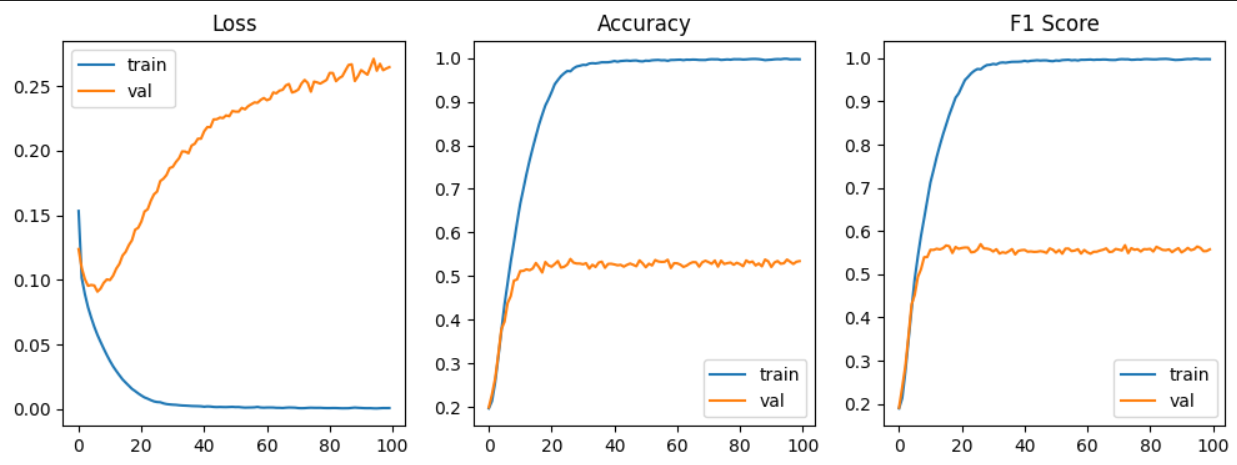
\includegraphics[width=0.5\linewidth]{graphs.png}
    \caption{Metrics graphs for basic GRU model}
    \label{fig:enter-label}
\end{figure}

This basic architecture resulted in overfitting, as evidenced by the training and validation metrics.

\subsection{Test set results}



\subsection{Improvement}

\begin{itemize}
    \item \textbf{GloVe Embeddings}: Pre-trained GloVe 100 embeddings were used to create an embedding matrix for the vocabulary.
    \item \textbf{Improved GRU Model}: An improved GRU model is defined, which uses the pre-trained GloVe embeddings, a dropout layer (0.2), and a higher learning rate (from 0.0005 to 0.001)
    \item Training was for 200 epochs
\end{itemize}

\begin{figure}
    \centering
    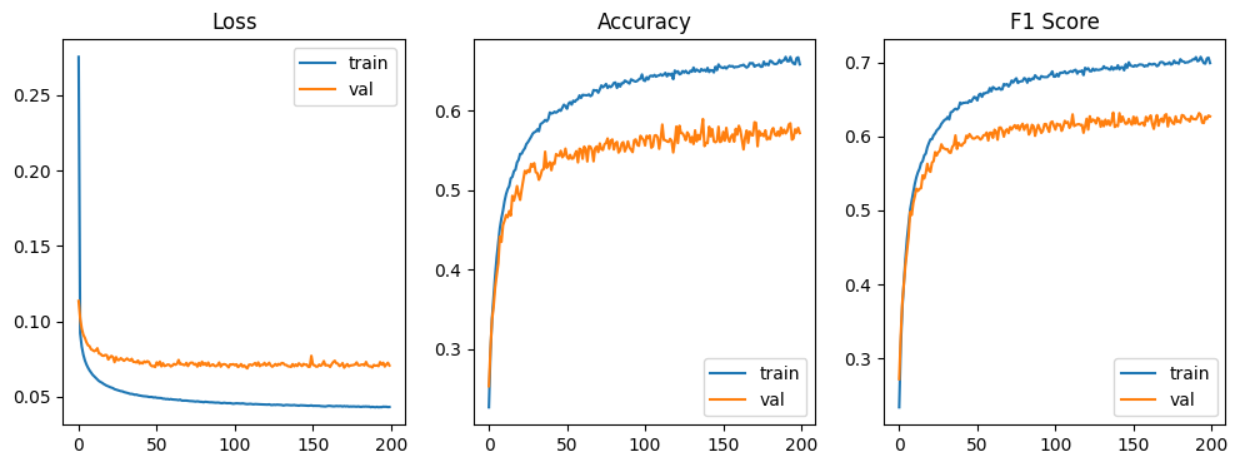
\includegraphics[width=0.5\linewidth]{improved_graphs.png}
    \caption{Metrics graphs of improved GRU}
    \label{fig:enter-label}
\end{figure}

The improved architecture, helped avoid overfitting but validation loss and accuracy almost remained the same

\subsection{Final results on test set}

\begin{table}[h]
\centering
\begin{tabular}{|l|c|c|c|}
\hline
\textbf{Model} & \textbf{Test Loss} & \textbf{Test Acc} & \textbf{Test F1} \\
\hline
GRUModel & 0.2744 & 0.4796 & 0.4976 \\
ImprovedGRUModel & 0.0743 & 0.5552 & 0.6034 \\
\hline
\end{tabular}
\caption{Evaluation Results of GRU Models}
\label{tab:gru_results}
\end{table}
\end{document}